\documentclass{article}
\usepackage{graphicx} % Required for inserting images
\usepackage{circuitikz} % for logic gates
\usetikzlibrary{shapes.geometric}
\usepackage{amsmath}
\usepackage{microtype}

\title{Quantum IS Exercises 1}
\author{Aman Mekas}
\date{August 2026}

\begin{document}

\maketitle

\begin{enumerate}
    \item[Exercise 1.1] How many possible states do (a) four coins have? (b) five coins? You do not need to list the states, just how many there are.
    \begin{enumerate}
    \item[a)]\(2^4 = 16\)
    \item[b)]\(2^5 = 32\)\newline
    \end{enumerate}


    \item[Exercise 1.2] How many possible states do (a) four dice have? (b) five dice? You do not need to list the states, just how many there are. A calculator may be useful.
    \begin{enumerate}
    \item[a)]\(6^4 = 1296\)
    \item[b)]\(6^5 = 7776\)\newline
    \end{enumerate}


    \item[Exercise 1.3] Some board games use a twenty-sided die. How many twenty-sided dice does it take to encode the seven colors of the rainbow?
    \begin{enumerate}
    \item[a)] Just one.\newline
    \end{enumerate}


    \item[Exercise 1.4] How many (a) coins and (b) six-sided dice would it take to represent the 26 letters of the English alphabet. Ignore upper and lowercase, spaces, punctuation, etc., so there's only 26 letters total.
    \begin{enumerate}
    \item[a)] It would take 5 coins. \(2^5 = 32\) and \(32>26\), so there are enough combinations.
    \item[b)] It would take just two dice. \(6^2 = 36\) and \(36>26\), so there are enough combinations. Note: I am doing \(6^n\) for any \(n\) combinations because there are 6 possibilities.\newline
    \end{enumerate}


    \item[Exercise 1.5] Convert the following binary numbers (base 2) to decimal numbers (base 10): (a) \(10111_2\) and (b) \(11001010_2\).
    \begin{enumerate}
    \item[a)] \((1\cdot2^0)+(1\cdot2^1)+(1\cdot2^2)+(0\cdot2^3)+(1\cdot2^4)\) = \(1 + 2 + 4 + 0 + 16 = 23\)
    \item[b)] \((0\cdot2^0)+(1\cdot2^1)+(0\cdot2^2)+(1\cdot2^3)+(0\cdot2^4)+(0\cdot2^5)+(1\cdot2^6)+(1\cdot2^7)\) = \(0+2+0+8+0+0+64+128=202\)\newline
    \end{enumerate}

    \item[Exercise 1.6] Convert the following decimal numbers (base 10) to binary numbers (base 2): (a) 42 and (b) 495.
    \begin{enumerate}
    \item[a)] \(42-2^5=10\), \(10-2^3 = 2\), \(2-2^1=0\): \(42 = \boldsymbol{101010_2}\)
    \item[b)] \(495-2^8=239\), \(239-2^7=111\), \(111-2^6=47\), \(47-2^5=15\), \(15-2^3=7\), \(7-2^2=3\), \(3-2^1=1\), \(1-2^0=0\): \(495 = \boldsymbol{111101111_2}\)\newline
    \end{enumerate}

    \item[Exercise 1.7] Base-16, commonly called hexadecimal, is another frequently used number system in computing. The sixteen digits are 0, 1, 2, 3, 4, 5, 6, 7, 8, 9, A, B, C, D, E, F. So the letter A is ten in decimal, B is eleven in decimal, ..., and F is fifteen in decimal. For example, converting the hexadecimal number F2A to decimal,\newline
    \(F2A = 16^2\cdot F + 16^1\cdot2 +16^0\cdot A\)\newline
    \(= 256\cdot15 + 16\cdot2 + 1\cdot10\)\newline
    \(=3840+32+10\)\newline
    \(=3882.\)\newline
    
    (a) Convert the hexadecimal number 3B7C to a decimal (base 10) number.\newline
    (b) Convert the hexadecimal number FF to a binary (base 2) number. (So two hexadecimal numbers can represent eight bits.)\newline
    (c) HTML uses hexadecimal to encode colors using the RGB color model. RGB stands for the (additive) primary colors red, green, and blue, and by adding together different amounts of their light, the other colors can be produced. [From painting, you may be familiar with the (subtractive) primary colors, red, yellow, and blue.] The amount of red, green, and blue ranges from 0 to 255, with 0 being none of the color, and 255 being the full amount of the color. This range of 0 to 255 corresponds to the hexadecimal numbers 00 through FF. An HTML color code uses six hexadecimal numbers, like FA10E4, with the left two digits (FA) corresponding to the amount of red, the middle two digits (10) corresponding to the amount of green, and the right two digits (E4) corresponding to the amount of blue. This particular mix of colors results in a bright pink. Convert the hexadecimal numbers FA, 10, and E4 to decimal.

    \begin{enumerate}
    \item[a)] \(16^3\cdot3 + 16^2\cdot11 + 16^1\cdot7 + 16^0\cdot12 = 15,228\)
    \item[b)] \(FF = 11111111\). This is because F = 15 and 15 in binary is 1111. Therefore, \(FF = \boldsymbol{11111111}\)
    \item[c)] \(FA = 16^1\cdot15 + 16^0\cdot10 = \boldsymbol{250}\)\newline
    \(10 = 16^1\cdot1 + 16^0\cdot0 = \boldsymbol{16}\)\newline
    \(E4 = 16^1\cdot14 + 16^0\cdot4 = \boldsymbol{228}\)\newline
    \end{enumerate}

    \item[Exercise 1.8] Negative numbers can be encoded in binary using two’s complement, where the most significant bit is negative, while the remaining bits are positive. For example, in two’s complement,\newline
    
    \(11010_2 = 1\cdot(-2^4) + 1\cdot2^3 + 0\cdot2^2 + 1\cdot2^1 + 0\cdot2^0 = -6\). \newline
    
    Convert each of the following two’s complement numbers to decimal:\newline

    \begin{displaymath}
        \begin{array}{|c c|}
             \hline
             \text{Binary Decimal} & \text{Two's Complement (Base 10)}  \\
             \hline
             000 & ? \\
             001 & ? \\
             010 & ? \\
             011 & ? \\
             100 & ? \\
             101 & ? \\
             111 & ? \\
             \hline
        \end{array}
    \end{displaymath}
    \newline
    \begin{enumerate}
    \item[a)] 
    \begin{displaymath}
        \begin{array}{|c c|}
             \hline
             \text{Binary Decimal} & \text{Two's Complement (Base 10)}  \\
             \hline
             000 & 0 \\
             001 & 1 \\
             010 & 2 \\
             011 & 3 \\
             100 & -4 \\
             101 & -3 \\
             111 & -1 \\
             \hline
        \end{array}
    \end{displaymath}
    \end{enumerate}


    \item[Exercise 1.9] Write your first name as an ASCII bit string.
    \begin{enumerate}
    \item[a)] \(1000001\hspace{0.08in}1101101\hspace{0.08in}1100001\hspace{0.08in}1101110\)\newline
    \end{enumerate}

    \item[Exercise 1.10] Decode the following ASCII characters: \newline
    \(1010001\hspace{0.08in}1110101\hspace{0.08in}1100001\hspace{0.08in}1101110\hspace{0.08in}1110100\hspace{0.08in}1110101\hspace{0.08in}1101101\)
    \begin{enumerate}
    \item[a)] Quantum
    \end{enumerate}
        
    \item[Exercise 1.11] Consider the following gate that inverts the inputs before passing them into an or gate, sometimes called a $\textit{negative-OR gate:}$\newline  
    
    \begin{circuitikz}[american]
      % 1. Place the standard American OR gate
      \draw (0,0) node[or port] (myOR) {};
      % 2. Extend input wires to the left, add bubbles at the end, and push labels outward
      \draw (myOR.in 1) -- ++(-0.4,0) node[ocirc] {} node[left=4pt] {A};
      \draw (myOR.in 2) -- ++(-0.4,0) node[ocirc] {} node[left=4pt] {B};
      % 3. Place output label
      \node[right] at (myOR.out) {$\bar A +\bar B$};
    \end{circuitikz}\newline
    
    (a) Write the truth table for this circuit.\newline
    (b) What logic gate is this equivalent to?
    \begin{enumerate}
        \item[a)]
        \begin{displaymath}
            \begin{array}{|c c|c|}
                 A & B & \bar A + \bar B  \\
                 F & F & T \\
                 F & T & T \\
                 T & F & T \\
                 T & T & F \\
            \end{array}
        \end{displaymath}

        \item[b)] Logically equivalent to an NAND gate.
    \end{enumerate}

    \item[Exercise 1.12] Consider the following gate that inverts the inputs before passing them into an AND gate, sometimes called a $\textit{negative-AND gate:}$\newline

    \begin{circuitikz}[american]
      % 1. Place the standard American OR gate
      \draw (0,0) node[and port] (myAND) {};
      % 2. Extend input wires to the left, add bubbles at the end, and push labels outward
      \draw (myAND.in 1) -- ++(-0.4,0) node[ocirc] {} node[left=4pt] {A};
      \draw (myAND.in 2) -- ++(-0.4,0) node[ocirc] {} node[left=4pt] {B};
      % 3. Place output label
      \node[right] at (myOR.out) {$\bar A\bar B$};
    \end{circuitikz}\newline

    (a) Write the truth table for this circuit.\newline
    (b) What logic gate is this equivalent to?
    \begin{enumerate}
        \item[a)]
        \begin{displaymath}
            \begin{array}{|c c|c|}
                 A & B & \bar A \bar B  \\
                 F & F & T \\
                 F & T & F \\
                 T & F & F \\
                 T & T & F \\
            \end{array}
        \end{displaymath}
    \item[b)] Logically equivalent to a NOR gate.
    \end{enumerate}


    \item[Exercise 1.13] Consider the following electrical circuit:\newline
    
    \begin{circuitikz}[american, scale=1.2]
      % 1. Draw top and bottom connecting wires (bus lines)
      \draw (0,4) -- (4,4);
      \draw (0,0) -- (4,0);
      
      % 2. Left Branch: Standard DC Battery Source
      \draw (0,4) to[battery] (0,0);
      
      % 3. Middle Branch: Two Open Switches
      \draw (2,4) to[nos, a={$A=0$}] (2,2.2) 
                  -- (2,1.8) 
                  to[nos, a={$B=0$}] (2,0);
                  
      % 4. Right Branch: Vertical wire line
      \draw (4,4) -- (4,0);
      
      % 5. Clean circle overlay (replaces the 'lamp' to remove the X)
      \node[circle, draw, minimum size=0.7cm, fill=white, font=\large\bfseries] (bulb) at (4,2) {?};
      
      % 6. Output label positioned cleanly to the right of the circle
      \node[right=6pt] at (bulb.east) {Output = ?};
    \end{circuitikz}\newline

    Answer the following questions:\newline

    (a) Say A = 0 and B = 0. Sketch the circuit and draw arrows indicating the path through which the electricity is flowing. Is the light bulb off or on?\newline
    (b) Say A = 0 and B = 1. Sketch the circuit and draw arrows indicating the path through which the electricity is flowing. Is the light bulb off or on?\newline
    (c) Say A = 1 and B = 0. Sketch the circuit and draw arrows indicating the path through which the electricity is flowing. Is the light bulb off or on?\newline
    (d) Say A = 1 and B = 1. Sketch the circuit and draw arrows indicating the path through which the electricity is flowing. Is the light bulb off or on?\newline
    (e) What logic gate does the circuit correspond to?
    
    \begin{enumerate}
        \item[a)] The light bulb is on. The electricity flows through the bulb because the middle path is closed.
        \item[b)] The light bulb is still on. Even though B = 1, the electricity will still flow through the bulb, because it has the least resistance (technically.)
        \item[c)] The light bulb is still on. Even though A = 1, the electricity will still flow through the bulb, because it has the least resistance (technically.)
        \item[d)] If both A and B = 1, then the light bulb will most likely not turn on. This is because electricity tends to flow through the path of least resistance, therefore, because the wire has no resistance (theoretically) the bulb will not be on.
        \item[e)] This corresponds to the NAND logic gate, because the bulb is on in every instance except for when both A and B are true.
    \end{enumerate}

    \item[Exercise 1.14] Consider the following electrical circuit:\newline
    
    \begin{circuitikz}[american, scale=1.2]
      % 1. Draw top and bottom connecting wires (bus lines)
      \draw (0,0) -- (6,0);
      \draw (0,0) -- (0,4);
      
      % 2. Left Branch: Standard DC Battery Source
      \draw (6,4) to[battery] (0,4);
      
      % 3. Middle Branch: Two Open Switches
      \draw (4,4) to[nos, a={$A=0$}] (4,0);

      \draw (6,4) to [nos, a={$B=0$}] (6,0);
      
      
      % 5. Clean circle overlay (replaces the 'lamp' to remove the X)
      \node[circle, draw, minimum size=0.7cm, fill=white, font=\large\bfseries] (bulb) at (0,2) {?};
      
      % 6. Output label positioned cleanly to the right of the circle
      \node[right=6pt] at (bulb.east) {Output = ?};
    \end{circuitikz} \newline

    Answer the following questions:\newline
    (a) Say A = 0 and B = 0. Sketch the circuit and draw arrows indicating the path through which the electricity is flowing. Is the light bulb off or on?\newline
    (b) Say A = 0 and B = 1. Sketch the circuit and draw arrows indicating the path through which the electricity is flowing. Is the light bulb off or on?\newline
    (c) Say A = 1 and B = 0. Sketch the circuit and draw arrows indicating the path through which the electricity is flowing. Is the light bulb off or on?\newline
    (d) Say A = 1 and B = 1. Sketch the circuit and draw arrows indicating the path through which the electricity is flowing. Is the light bulb off or on?\newline
    (e) What logic gate does the circuit correspond to?

    \begin{enumerate}
        \item[a)] If both A and B are 0, then the electricity cannot flow through the circuit to reach the bulb, therefore the bulb will be off.
        \item[b)] If A is 0 and B = 1, then the electricity can flow through either channel, meaning that the bulb will be on.
        \item[c)] If A is 1 and B = 0, then the electricity can flow through either channel, meaning that the bulb will be on.
        \item[d)] If both A and B are 1, then the electricity can flow through both channels equally, meaning that the bulb will be on.
        \item[e)] This circuit corresponds with an OR logic gate.
    \end{enumerate}


    \item[Exercise 1.15] Consider the following electrical circuit:\newline
    
    \begin{circuitikz}[american, scale=1.2]
      % 1. Draw top and bottom connecting wires (bus lines)
      \draw (0,0) -- (6,0);
      \draw (0,4) -- (6,4);
      \draw (6,0) -- (6,4);
      
      % 2. Left Branch: Standard DC Battery Source
      \draw (0,4) to[battery] (0,0);
      
      % 3. Middle Branch: Two Open Switches
      \draw (2,4) to[nos, a={$A=0$}] (2,0);

      \draw (4,4) to [nos, a={$B=0$}] (4,0);
      
      
      % 5. Clean circle overlay (replaces the 'lamp' to remove the X)
      \node[circle, draw, minimum size=0.7cm, fill=white, font=\large\bfseries] (bulb) at (6,2) {?};
      
      % 6. Output label positioned cleanly to the right of the circle
      \node[right=6pt] at (bulb.east) {Output = ?};
    \end{circuitikz}\newline

    Answer the following questions:\newline
    (a) Say A = 0 and B = 0. Sketch the circuit and draw arrows indicating the path through which the electricity is flowing. Is the light bulb off or on?\newline
    (b) Say A = 0 and B = 1. Sketch the circuit and draw arrows indicating the path through which the electricity is flowing. Is the light bulb off or on?\newline
    (c) Say A = 1 and B = 0. Sketch the circuit and draw arrows indicating the path through which the electricity is flowing. Is the light bulb off or on?\newline
    (d) Say A = 1 and B = 1. Sketch the circuit and draw arrows indicating the path through which the electricity is flowing. Is the light bulb off or on?\newline
    (e) What logic gate does the circuit correspond to?

    \begin{enumerate}
        \item[a)] If A and B are 0, then the electricity flows through the bulb, meaning that the bulb is on.
        \item[b)] If A = 0 and B = 1, then the electricity flows through the open channel (B) because it is the path of least resistance, meaning that the bulb is off.
        \item[c)] If A = 1 and B = 0, then the electricity flows through the open channel (A) because it is the path of lest resistance, meaning that the bulb is off.
        \item[d)] If A and B are 1, then the electricity equally flows through the open gates, meaning that the bulb is off.
        \item[e)] This circuit corresponds with a NOR gate.
    \end{enumerate}


    \item[Exercise 1.16] Consider the following electrical circuit:\newline
    
    \begin{circuitikz}[american, scale=1.2] \newline
      % 1. Left Branch: DC Battery Source (Lowered to clear everything)
      \draw (0,3) to[battery] (0,0);
      \draw (0,3)--(1.8,3);
    
      \draw[dashed] (1.6,1.6) rectangle (3.4,4.0);
      \node[above] at (2.5,4.0) {Switch A};
      
      \fill (1.8,3) circle (1.5pt);
      \node[below=5pt] at (1.8,3) {C};
      \fill (3.0,3.5) circle (1.5pt);
      \node[above=4pt] at (3.0,3.5) {0};
      \fill (3.0,2.3) circle (1.5pt);
      \node[below=4pt] at (3.0,2.3) {1};
      
      \draw[-latex, thick] (1.8,3) -- (2.9,3.45);
      
    
      \draw[dashed] (4.4,1.6) rectangle (6.2,4.0);
      \node[above] at (5.3,4.0) {Switch B};
      
      \fill (4.6,3.5) circle (1.5pt);
      \node[above=4pt] at (4.6,3.5) {0};
      \fill (4.6,2.3) circle (1.5pt);
      \node[below=4pt] at (4.6,2.3) {1};
      \fill (5.8,3) circle (1.5pt);
      \node[below=5pt] at (5.8,3) {C};
      
      \draw[-latex, thick] (4.7,2.35) -- (5.8,3);
    
      \draw (3.0,3.5) -- (4.6,2.3);
      \draw (3.0,2.3) -- (4.6,3.5);
    
      \draw (5.8,3) -- (7.5,3) -- (7.5,2.35);
      
      \foreach \angle in {45, 90, 135, 225, 270, 315} {
        \draw (7.5,2) +(\angle:0.35cm) -- +(\angle:0.55cm);
      }
      
      \node[circle, draw, minimum size=0.7cm, fill=white, font=\small\bfseries] (bulb) at (7.5,2) {On};
      
      \draw (7.5,1.65) -- (7.5,0) -- (0,0);
      
      \node[right=12pt] at (bulb.east) {-- Output = 1};
    
    \end{circuitikz} \newline


    Each switch has three poles, labeled C, 0, and 1. Switch A is current flipped up, which connects C and 0. Switch B is currently flipped down, which connects C and 1. In this configuration, there is a complete path for the electricity to flow. It comes out of the positive end of the battery, through Switch A along A = 0, then down to B = 1, then through Switch B, then down through the light bulb, left through the bottom wire, and up to the negative end of the battery. So, the light bulb is on when A = 0 and B = 1.\newline

    Answer the following questions:\newline
    (a) Say A = 0 and B = 0. Sketch the circuit and draw arrows indicating the path through which the electricity is flowing. Is the light bulb off or on?\newline
    (b) Say A = 1 and B = 0. Sketch the circuit and draw arrows indicating the path through which the electricity is flowing. Is the light bulb off or on?\newline
    (c) Say A = 1 and B = 1. Sketch the circuit and draw arrows indicating the path through which the electricity is flowing. Is the light bulb off or on?\newline
    (d) What logic gate does the circuit correspond to?

    \begin{enumerate}
        \item[a)] If A = 0 and B = 0, then the flow of electricity doesn't connect. Therefore, the bulb is off.
        \item[b)] If A = 1 and B = 0, then the flow of electricity connects. Therefore, the bulb is on.
        \item[c)] If A = 1 and B = 1, then the flow of electricity doesn't connect. Therefore, the bulb is off.
        \item[d)] The circuit corresponds to an XOR logic gate.
    \end{enumerate}


    \item[Exercise 1.17] Visit the website https://en.wikipedia.org/wiki/Transistor\_count.\newline
    (a) Pick an older computer processor. Which one did you pick, what year was it introduced, and how many transistors did it have?\newline
    (b) Pick a newer computer processor. Which one did you pick, what year was it introduced, and how many transistors did it have?
    \begin{enumerate}
        \item[a)] Intel 4004 (4-bit, 16-pin) 1971 has 2,250 transistors
        \item[b)] NVIDIA Vera (multi-chip module, 88-cores 64-bit Armv9.2, 176MB L2 + 162MB L3 cache) 2026 has 227,000,000,000 transistors.
    \end{enumerate}


    \item[Exercise 1.18] Consider the XOR of three bits A, B, and C, which can either be two two-bit XOR gates strung together, or a single three-bit XOR gate:\newline
    (a) What is the truth table for this circuit?\newline
    (b) When there is an even number of 1’s in the input (we call this even parity), what is the output?\newline
    (c) When there is an odd number of 1’s in the input (we call this odd parity), what is the output?
    \begin{enumerate}
        \item[a)] Truth table:

        \begin{displaymath}
            \begin{array}{|c c c|c|c|}
                 \hline
                 A & B & C & A\oplus B & A\oplus B\oplus C  \\
                 \hline
                 F & F & F & F & F \\
                 F & F & T & F & F \\
                 F & T & F & T & T \\
                 F & T & T & T & F \\
                 T & F & F & T & T \\
                 T & F & T & T & F \\
                 T & T & F & F & F \\
                 T & T & T & F & T \\
                 \hline
            \end{array}
        \end{displaymath}
    \end{enumerate}

\begin{figure}
    \centering
    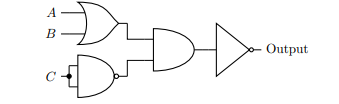
\includegraphics[width=0.5\linewidth]{Screenshot 2026-09-09 8.28.09 AM.png}
    \caption{ex. 1.19}
\end{figure}

\item[Exercise 1.20] Answer the following questions:\newline
(a) How many possible one-bit logic gates are there?\newline
(b) How many possible two-bit logic gates are there?\newline
(c) How many possible three-bit logic gates are there?\newline
(d) How many possible four-bit logic gates are there?\newline
(e) How many possible n-bit logic gates are there?\newline
\begin{enumerate}
    \item[a)] \(2^2 = 4\)
    \item[b)] \(2^4=16\)
    \item[c)] \(2^8=256\)
    \item[d)] \(2^16=65536\)
    \item[e)]  \(2^{2^n}\)
\end{enumerate}

\item[Exercise 1.21] Draw a circuit diagram using only NOT, AND, and OR gates that implements the XOR gate.]\newline
\begin{enumerate}
    \item[a)]

    \begin{circuitikz}[american]
      % 1. Place the standard American OR gate
      \draw (0,0) node[or port] (myOR) {};
      % 2. Extend input wires to the left, add bubbles at the end, and push labels outward
      \draw (myOR.in 1) -- ++(-0.4,0) node[ocirc] {} node[left=4pt] {A};
      \draw (myOR.in 2) -- ++(-0.4,0) node[ocirc] {} node[left=4pt] {B};
      % 3. Place output label
      \node[right] at (myOR.out) {$\bar A +\bar B$};
    \end{circuitikz}
    
\end{enumerate}


\item[Exercises 1.30] Changing the OR to an XOR does not change the logic, so the truth table stays the same.

\item[Exercises 1.31] 10000 or 16

\item[Exercises 1.32] 11100110

\item[Exercises 1.33] 10100 or 20

\item[Exercises 1.34] A + B

\item[Exercises 1.35] \(A + \neg(B+C)\)

\item[Exercises 1.36] \(ABC + \neg ABC + AB\neg C = B(A+C)\)

\item[Exercises 1.46](a) \(2^{13}\) = 8192. (b) spontaneously flip, Radioactive atoms, presence, absense, single event upset. (c) miniaturized. (d) increased, greater, sky (e) cosmic rays, particles, black holes. (f) cascade, transistor. (g) error correction code. (h) month, cosmic rays. (i) 10 to 30. (j) 161. (k) flash, every star.

\item[Exercises 1.47](a) Even. (b) No. (c) Yes. The parity of the first seven bits doesn’t match the parity bit. (d) No. If two bits flipped, the parity would be unchanged.


\item[Exercises 1.48] (a) Yes, the middle bit has flipped. (b) Yes, the left bit has flipped. (c) 0.1040. Decrease, since 0.1040 < 0.2. (d) 0.7840. Increase, since 0.78404 > 0.7.

\item[Exercises 1.50] (a) f(100). (b) g(500). (c) They are equal when n = 477, after which g(n) is greater than f(n). (d) true, true, false, false, false.


\item[Exercises 1.51] Possibilities are (a) iii or v, (b) i or v, (c) ii or v, (d) v, (e) i or iv. Thus, the only correct answer is (a) iii, (b) i, (c) ii, (d) v, (e) iv.

\item[Exercises 1.52] (a) Efficient. (b) Efficient. (c) Efficient. (d) Inefficient. (e) Inefficient. (f) Inefficient.

\item[Exercises 1.53] (a) Bounded-Error Probabilistic Polynomial-Time. (b) “As the class of feasible problems for a computer with access to a genuine random-number source.”

\item[Exercises 1.54] Many possible answers, including factoring, graph isomorphism, n x n Sudoku, traveling salesman, Hamiltonian path, and bin packing.

\item[Exercises 1.55] (a) Yang–Mills and Mass Gap, Riemann Hypothesis, P vs NP Problem, Navier–Stokes Equation, Hodge Conjecture, Poincare Conjecture, and Birch and Swinnerton-Dyer Conjecture. Only the Poincare Conjecture is solved. (b) Stephen
Cook and Leonid Levin in 1971.

\item[Exercises 1.56]Answers vary.
    
\end{enumerate}

\end{document}
